% Full twenty-sheet observations supplied by the parent review; the three
% illustrated source/seed sheets were also inspected during figure preparation.
\subsection{Request-Conditioned Memory}
\label{sec:r83-completed}
\subsubsection{Completed design and matched comparison population}
We compare seven memory and correction configurations on the same ten seen development sources, one per official category, with two seeds per source. REQUEST\_MEMORY, REQUEST\_BOTH, and MEAN\_MEMORY vary memory allocation; U25\_KV, FlowEdit N26, SOFT75, and REQUEST\_SOFT25 (memory-fixed) provide references matched on source, task, seed, and prompts.

Let $E$ be the native request-response map and $P=1-0.75E$ its protection weight. Three memory-off reference states each receive one source-prompt and one target-prompt evaluation, giving six native transformer probes. Average pooling over the same $2\times2$ latent patches used by FLUX packing maps $P$ from the $64\times64$ spatial grid to query weights $P_q$ on the $32\times32$ token grid. REQUEST\_MEMORY multiplies the inherited query-memory gate by $P_q$ while retaining global quarter-strength correction. REQUEST\_BOTH combines this spatial memory multiplier with request-routed ONLINE correction. MEAN\_MEMORY uses the same request-routed correction and replaces $P_q$ with its spatial mean. Source K/V pools, target-text contribution, attention blocks, and the first seven active memory steps remain fixed.

The mean control isolates spatial allocation from average memory attenuation. The recorded mean multiplier is identical between REQUEST\_BOTH and MEAN\_MEMORY in every paired slot, averaging 0.7359 across records. Their realized step-averaged gate values differ by at most 0.00046. This control matches the mean query multiplier; attention energy and the subsequent edited trajectories remain measured consequences of the allocation.

\subsubsection{Pixel measurements and source-level estimates}
Archived pixel measurements compare generated outputs with the source on a $512\times512$ grid. Whole-image NCC is source correlation. Its boundary-spanning crop permits only zero displacement, so fixed and shift-search NCC coincide. Global and edit-region MAE cover all ten sources. Preservation MAE uses eight sources and sixteen records per configuration: the lemon-addition source 223000000008 and crayon-style source 922000000003 have empty preservation complements. Those observations remain missing for this metric.

\begin{table*}[t]
\centering\footnotesize
\setlength{\tabcolsep}{4pt}
\caption{Completed memory study on the same ten seen development sources and two seeds. Every row contains twenty records. Preservation MAE uses eight eligible sources; the other pixel metrics use ten. Edit-region MAE measures source departure. Times describe recorded executions. REQUEST\_SOFT25 (memory-fixed) retains the original all-query memory.}
\label{tab:r83-means}
\begin{tabular}{lrrrrrr}
\toprule
Configuration & Global MAE & Whole NCC $\uparrow$ & Preservation MAE $\downarrow$ & Edit MAE & NFE & Time (s)\\
\midrule
REQUEST\_MEMORY & 0.1318 & 0.7444 & 0.1148 & 0.1491 & 97 & 55.63\\
REQUEST\_BOTH & 0.1296 & 0.7255 & 0.1093 & 0.1589 & 97 & 45.58\\
MEAN\_MEMORY & 0.1316 & 0.7221 & 0.1095 & 0.1581 & 97 & 45.80\\
U25\_KV & 0.1250 & 0.7635 & 0.1114 & 0.1380 & 91 & 43.38\\
FlowEdit N26 & 0.1271 & 0.7163 & 0.1032 & 0.1645 & 52 & 30.78\\
SOFT75 & 0.1273 & 0.7668 & 0.1147 & 0.1384 & 91 & 43.71\\
\shortstack[l]{REQUEST\_SOFT25\\(memory-fixed)} & 0.1227 & 0.7446 & 0.1060 & 0.1464 & 97 & 45.42\\
\bottomrule
\end{tabular}
\end{table*}

For each comparison, we first average paired differences over the two seeds within a source, then give each source equal weight. Percentile 95\% intervals use 20,000 bootstrap resamples of source means. Table~\ref{tab:r83-pairs} reports exploratory intervals without multiple-comparison adjustment.

\begin{table}[t]
\centering\scriptsize
\caption{Source-paired differences, first configuration minus reference. MAE uses normalized RGB values. NCC uses the whole image. Each cell gives mean difference and source-bootstrap 95\% interval. Preservation uses eight source clusters; other columns use ten. BOTH, MEAN, and MEMORY denote REQUEST\_BOTH, MEAN\_MEMORY, and REQUEST\_MEMORY; REQ denotes REQUEST\_SOFT25 (memory-fixed); MEM denotes REQUEST\_MEMORY.}
\label{tab:r83-pairs}
\setlength{\tabcolsep}{2pt}
\begin{tabular}{lrrr}
\toprule
Comparison & Whole NCC & Pres. MAE & Edit MAE\\
\midrule
BOTH $-$ MEAN & \shortstack{$0.0034$\\$[-0.0041,0.0127]$} & \shortstack{$-0.0003$\\$[-0.0020,0.0012]$} & \shortstack{$0.0008$\\$[-0.0051,0.0050]$}\\
MEM $-$ U25 & \shortstack{$-0.0191$\\$[-0.0321,-0.0077]$} & \shortstack{$0.0034$\\$[0.0003,0.0077]$} & \shortstack{$0.0112$\\$[0.0060,0.0170]$}\\
BOTH $-$ REQ & \shortstack{$-0.0191$\\$[-0.0298,-0.0095]$} & \shortstack{$0.0033$\\$[0.0001,0.0076]$} & \shortstack{$0.0125$\\$[0.0072,0.0183]$}\\
\bottomrule
\end{tabular}
\end{table}

\subsubsection{Spatial allocation and memory release}
REQUEST\_BOTH minus MEAN\_MEMORY gives a whole-image NCC difference of $0.0034$, with interval $[-0.0041,0.0127]$; six sources increase and four decrease. Preservation MAE differs by $-0.0003$, with interval $[-0.0020,0.0012]$, with three sources improving and five worsening. The estimates are small and uncertain: the intervals allow effects in either direction, and no equivalence margin was specified. They leave the value of spatial placement relative to mean attenuation open.

REQUEST\_MEMORY increases preservation MAE by 0.0034 relative to U25 and reduces NCC by 0.0191. Six of eight sources have greater preservation error, and nine of ten have lower NCC. With request-routed correction already present, REQUEST\_BOTH increases preservation MAE by 0.0033 and reduces NCC by 0.0191 relative to REQUEST\_SOFT25 (memory-fixed), with the same source-level directions. Edit-region departure increases on every source in both comparisons. These pixel results locate additional change inside and outside the official edit regions. Its value for the requested transformation depends on the task, as illustrated by the style improvement and relational failures below.

\noindent\textbf{Post hoc sensitivity of the memory comparison.}
For the archived ten-source spatial-minus-mean whole-image NCC difference, the mean is $0.0034$. Removing the crayon source, whose source-level difference is $0.0377$, gives $-0.0004$ across the remaining nine sources. This post hoc analysis shows sensitivity to source composition; the primary estimate retains all ten sources.

\subsubsection{Visible style gains and persistent relational errors}
The qualitative review covered all twenty paired comparison sheets across both seeds. Figure~\ref{fig:r83-memory-examples} displays three source--seed cases with the original delivered previews and a common column order. In the crayon-style case at seed 17, all three new configurations move toward a hand-drawn cartoon appearance. REQUEST\_BOTH shows a particularly clear drawn rendering of the face, hair, and shirt compared with REQUEST\_SOFT25 (memory-fixed). This is a positive, task-specific signal from memory release. MEAN\_MEMORY also strengthens the illustrated appearance but contains a conspicuous secondary face in the background. Spatial and mean memory attenuation can thus reach similar aggregate source correlations while differing in a visible artifact.

\begin{figure*}[t]
\centering
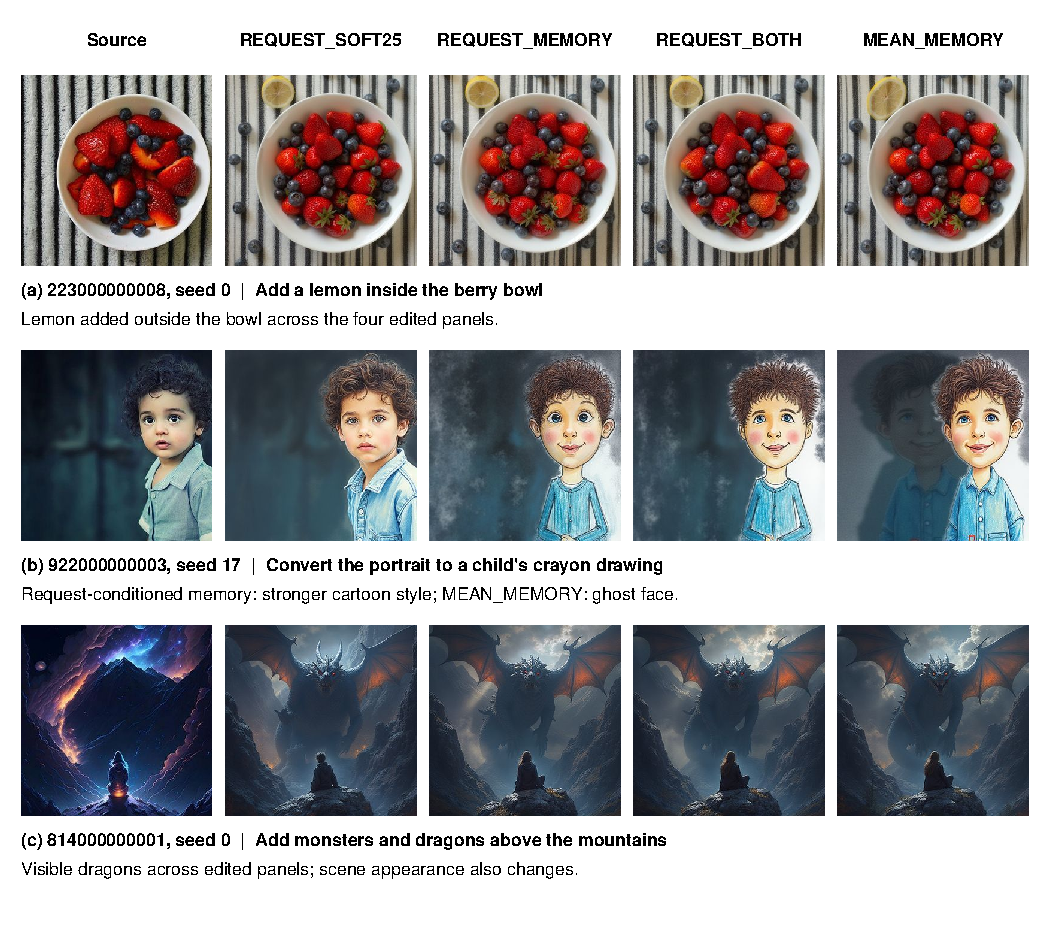
\includegraphics[width=.99\textwidth,height=.72\textheight,keepaspectratio]{figures/r83_memory_examples.pdf}
\caption{Completed request-memory examples. Columns: source, frozen REQUEST\_SOFT25 (memory-fixed), REQUEST\_MEMORY, REQUEST\_BOTH, and MEAN\_MEMORY. Top: source 223000000008, seed 0; the added lemon remains outside the berry bowl in all four edited panels. Middle: source 922000000003, seed 17; the three new configurations show stronger hand-drawn cartoon appearance, especially REQUEST\_BOTH, while MEAN\_MEMORY contains a ghost face. Bottom: source 814000000001, seed 0; every edited panel contains a visible dragon, with changes to the scene. Rows illustrate distinct requested outcomes and artifacts; labels occupy separate strips outside the image panels.}
\label{fig:r83-memory-examples}
\end{figure*}

Object presence and spatial relations remain distinct outcomes. In the lemon case at seed 0, all four displayed edited configurations add a lemon beside the bowl, leaving the requested inside relation unmet. The full review also finds the pepper still above the towel at seed 17 and transparent vessels remaining in the wooden-cup request at seed 0. The dragon example shows a visible requested addition across configurations, together with scene changes. These observations connect the increased edit-region departure to both useful stylistic change and persistent relational or material errors.

\subsubsection{Realized budgets and cost}
Each new configuration costs 97 standalone NFE: 28 inversion evaluations, 28 current-source evaluations, 28 target-generation evaluations, seven source-reference memory captures, and six native response probes. The probe count is identical for the mean control. Compared with U25's 91 NFE, the increase is six calls, or 6.6\%; REQUEST\_SOFT25 (memory-fixed) already uses 97 NFE.

Mean cumulative correction impulses are 0.2370 for REQUEST\_MEMORY, 0.2367 for REQUEST\_BOTH, and 0.2376 for MEAN\_MEMORY, versus 0.2319 for U25 and 0.2306 for REQUEST\_SOFT25 (memory-fixed). The ONLINE coefficient remains 0.25, with normalization errors below $1.6\times10^{-8}$ in the two new routed arms. The actual cumulative impulse varies with the edited trajectory. REQUEST\_BOTH and MEAN\_MEMORY average 45.58 and 45.80 seconds; run-level variability is documented in the provenance appendix.
